\chapter{Appendix}
\label{appendix}

\qquad The same dataset has been also projected onto 2D plane, as illustrated in the figure \ref{metrics-pca-13-to-2}.

\begin{figure}[htb]
	\centering
	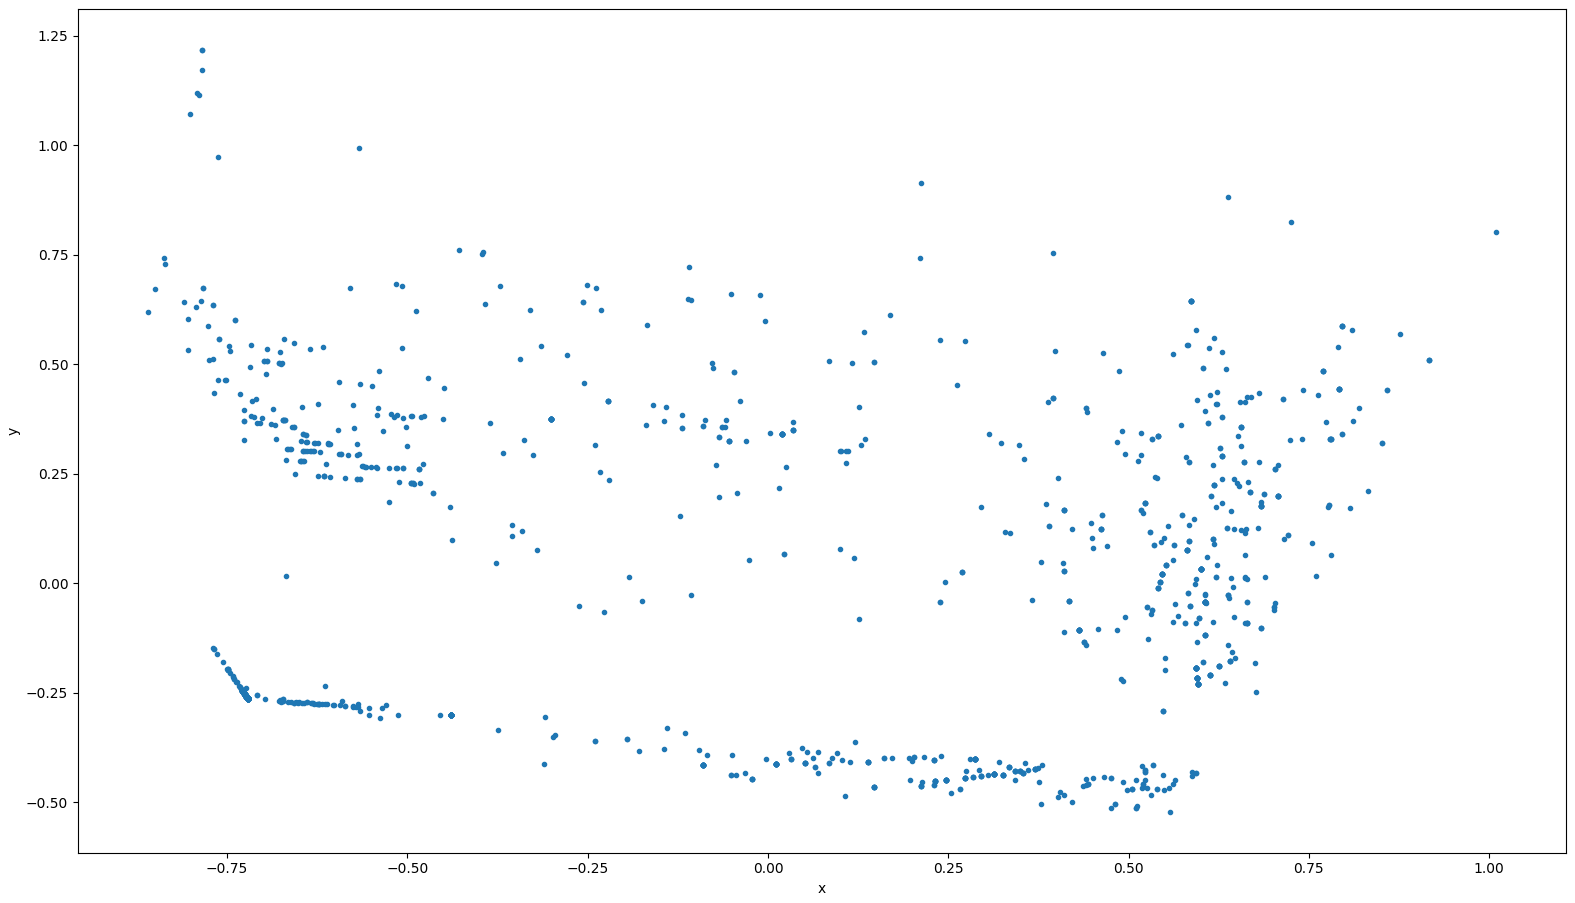
\includegraphics[width=\linewidth]{figs/metrics-pca-13-to-2.png}
	\caption{Visualisation of loop metrics dataset (13-dimensional metric vectors have been projected onto 2d space thanks to PCA algorithm) - blue dots correspond to metric values on single loops.}
	\label{metrics-pca-13-to-2}
\end{figure}
